\section{System Architecture}\label{sec:approach}
V7-B is the Python package \texttt{sbgv7}. A single \texttt{compare} invocation takes the two files, the entry, the inputs and a configuration, and writes an evidence log and a verdict. The modules are (Fig.~\ref{fig:arch}): a record layer (types, content-addressed ids, hash-chained JSONL log, trace), a boundary comparator, strict configuration validation, a child-side harness with monitoring-based line and branch capture, a runner (repeats, replay, activation), a pure decision function, an isolation layer, and a command-line entry point with a \texttt{verify} subcommand. Earlier-generation code (V5/V6) is untouched; only the changed-lines routine is imported read-only. The explorer (input generation), the internal-state module, S3 and Linux isolation are specified but not implemented.

\begin{figure}[t]\centering
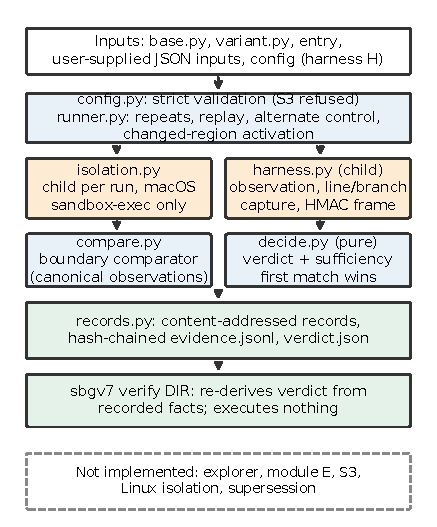
\includegraphics[width=0.92\columnwidth]{../../results/v7b_phase2_summary/figures/fig_p2_architecture.pdf}
\caption{V7-B modules and data flow (generated by \texttt{scripts/p2\_make\_paper\_figures.py}; no external diagram tool). Dashed box: specified but not implemented.}\label{fig:arch}
\end{figure}

For each input the runner executes each version $r_{det}=3$ times (early stop on disagreement); if the versions differ it performs $r_{replay}=5$ fresh replays per side and, if a controlled source was consulted, $k_{alt}=3$ alternate-control runs. Alternate runs virtualise seeded random, wall-clock functions based on \texttt{time.time}, and monotonic and performance counters, and seed \texttt{os.urandom} and \texttt{uuid4}; \texttt{datetime.now} and \texttt{secrets} are \emph{not} virtualised. The decision function then applies the verdict table of Section~\ref{sec:verdicts}.

\textbf{Implementation conformance status.} Against the 135 rules of the frozen specification the reconciled traceability matrix records 78 conforming, 30 partially conforming, 7 deviating, 14 not implemented, 2 unverifiable and 4 deferred to Phase 3 (78+30+7+14+2+4=135; \path{reports/phase2/PHASE2_TRACEABILITY_RECONCILIATION.md}). This is an implementation conformance status only. It says how much of a specification the code follows, not that the specification is right, that thresholds are calibrated, or that the system performs well. The unit tests executed with the E3 run were 286 passed and 1 skipped (\texttt{tests/v7} and \texttt{tests/v6}).

\textbf{Result channel.} The harness returns its result as one HMAC-authenticated frame on a dedicated pipe with a per-run key; a missing, duplicate, malformed or forged frame is a protocol violation that blocks both \DIV{} and \NDO{} (primary reason \texttt{unsafe\_program}). This is a local protocol-correctness fix, not a security boundary: the untrusted program shares the harness address space and can in principle recover the key.
